\chapter{Implementare}
\label{chapter:impl}

În acest capitol vom prezenta detaliile implementării acestui proiect. Se va 
trece prin structura de clase, fluxul datelor în aplicaţie, mutaţiile Modelului 
de Lucru (\ref{define:model})  şi funcţionarea componentelor de interfaţă, 
editorul OpenGL şi Vizualizarea 3D, prezentate în secţiunile 
\ref{section:opengl-editor}, respectiv \ref{section:view}.

Vom trece în revistă, de asemenea, principalele conexiuni la nivel de cod între 
componentele aplicaţiei, şi modul de interacţiune al principalelor module 
prezentate în Capitolul \ref{chapter:arh}.

Fiecare dintre componentele arhitecturale descrise la capitolul 
\ref{chapter:arh} sunt materializate în implementarea efectivă printr-un set de 
clase bine definite şi bine separate ca logică şi structură de celelalte 
componente ale aplicaţiei.

Există o diviziune clară între componentele abstracte, definitorii ale 
aplicaţiei noastre şi componentele materializate, implementările concrete. 
Toate abstracţiile făcute aici reprezintă forme de simplificare a 
interacţiunilor între obiecte, de marcare a anumitor comportamente şi separarea 
sarcinilor de dezvoltare în unităţi logice ce pot fi urmărite pe direcţia mai 
multor module de cod ale programului.

\section{Modelul de Lucru}

\subsection{Model}
Există o clasă specială pentru concretizarea conceptului de Model 
(\ref{define:model}). Responsabilităţile modelului cad în a fi un suport logic 
cît şi structural pentru obiectele ce materializează componentele modelului 
proiectat de către utilizator. Pentru asta, clasa model va şti întotdeauna 
diverse informaţii vitale funcţionării editorului.

Modelul în sine implementează aspectele de desenare pentru proiectate 
(\ref{define:editorRender}) şi de desenare reală (\ref{define:realRender}). 
Reutilizarea abstracţiei despre care vom vorbi imediat la Primitive conferă 
coerenţă şi creşte şi mai mult nivelul de abstactizare la care se poate lucra 
cu această aplicaţie.

Îndeplinirea sarcinilor de editare pentru proiectare şi de desenare reală se 
rezumă la apelarea aceloraşi rutine pentru toate componentele modelului. Pentru 
a reţine toate componentele, clasa de faţă reţine tabele de căutare pentru 
toate componentele care aleg să fie înregistrate în model.

Pot exista primitive care nu sunt desenate direct de către model, în speţă este 
cazul Caracteristicilor (\ref{define:feature}). Acestea sunt desenate de 
containerul lor, în speţă Zidul care le conţine.

Modelul serveşte şi ca suport pentru persistenţa datelor. Salvarea datelor în 
formatul specific aplicaţiei de faţă reprezintă varianta serializată a clasei 
model. De aceea, este important ca toate datele care sunt necesare salvării 
stării modelului să fie prezente cumva în legătură cu modelul, altfel există 
şansa ca ele să nu fie persistate de către aplicaţie în momentul în care se 
salvează în fişier documentul de lucru.

Modelul serveşte şi ca suport sumar de reţinere de stare pentru Editorul 
OpenGL. El va păstra în model selecţia curentă, cît şi starea transientă a 
unora dintre componente, cum ar fi dacă ele sunt navigate de către maus la 
momentul respectiv sau nu.

Aceasta se realizează prin păstrarea informaţiei despre elementele ce pot fi 
navigate (i.e. care implementează aspectul de Navigabilitate 
(\ref{define:hoverable})) într-o tabelă de căutare specială. Editorul va cere 
reevaluarea deciziei de navigabiltiate pentru toate componentele din această 
listă în momentul în care mausul îşi modifică poziţia în urma acţiunii 
utilizatorului.

\subsection{Primitive}
Clasa de bază a modelului de lucru este clasa Primitive. Desigur, este o 
materializare a conceptului de Primitivă (\ref{define:primitive}). Aceasta este 
o clasă abstractă care nu introduce nici un comportament singular, însă 
marchează nevoie de implementare pentru intefeţele EditorRenderable şi 
RealRenderable, necesare celor două vizualizări, cum vom vedea la secţiunile 
\ref{section:impl-editor} şi \ref{section:impl-view}.

Din clasa Primitive sunt extinse clasele concrete Corner, Wall şi toate clasele 
ce implementează Decoraţiunile (\ref{define:decoration}). Fiecare din aceste 
clase implementează metodele definite în interfeţele amintite mai sus.

Tot din clasa Primitive se desprinde şi clasa WallFeature, o materializare a 
conceptului de Caracterstică de Ziduri (\ref{define:feature}). Din ea la rîndul 
ei se concretizează clasele Door, Window, Inset, Outset, Tunnel, implementări 
ale diverselor caracteristici amintite în \ref{section:primitives}.

Deşi este doar o clasă de marcaj, Primitive prezintă un rol crucial în cadrul 
arhitecturii aplicaţiei noastre. Întreaga interacţiune pe care o au editorul şi 
vizualizarea 3D cu modelul se face prin această abstracţie. Tot ce are nevoie 
să ştie modelul despre orice componentă a sa este că extinde clasa Primitive. 
Cu această minimă funcţionalitate, se pot implementa toate operaţiile de 
desenare necesare interfeţei aplicaţiei de faţă.

\subsection{Corner}

Clasa Corner reprezintă una din puţinele Primitive care nu sunt direct 
disponibile utilizatorului aplicaţiei. Ea serveşte strict poziţionării 
Zidurilor şi prin aceasta editorul nu le oferă o importanţă deosebită printr-o 
individualizare în cadrul interfeţei, reducînd astfel solicitarea asupra curbei 
de învăţare a utilizatorului.

Clasa Corner, pe lîngă implementarea comportamentului de desenare pentru 
proiectate (\ref{define:editorRender}) şi de desenare reală 
(\ref{define:realRender}), aderă şi la comportamentele de Selectabilitate 
(\ref{define:selectable}) şi de Navigabilitate (\ref{define:hoverable}).

Ironic este însă că deşi joacă un rol atît de important în poziţionarea 
obiectelor în scenă, şi interacţionează mai mult decît orice altă componentă cu 
utilizatorul, colţurile nu au reprezentare specifică în editor. Deşi există un 
marcaj pentru starea de selecţie a colţului, în rest imaginea colţului este de 
fapt inexistentă. Îmbinarea lor cu alte componente şi efectul care îl au asupra
 Zidurilor îi oferă o reprezentare sugestivă şi pot fi controlate astfel de 
către utilizator.

\subsection{Wall}

Materializarea zidurilor are un rol important în cadrul aplicaţiei pentru că 
serveşte la rîndul său ca un container pentru toate tipurile de Caracteristici 
(\ref{define:feature}) ce pot fi adăugate în model. În acest scop, clasa reţine 
o listă sortată cu toate caracteristicile ce există pe acel Zid.

\begin{figure}[htp]
\begin{center}
  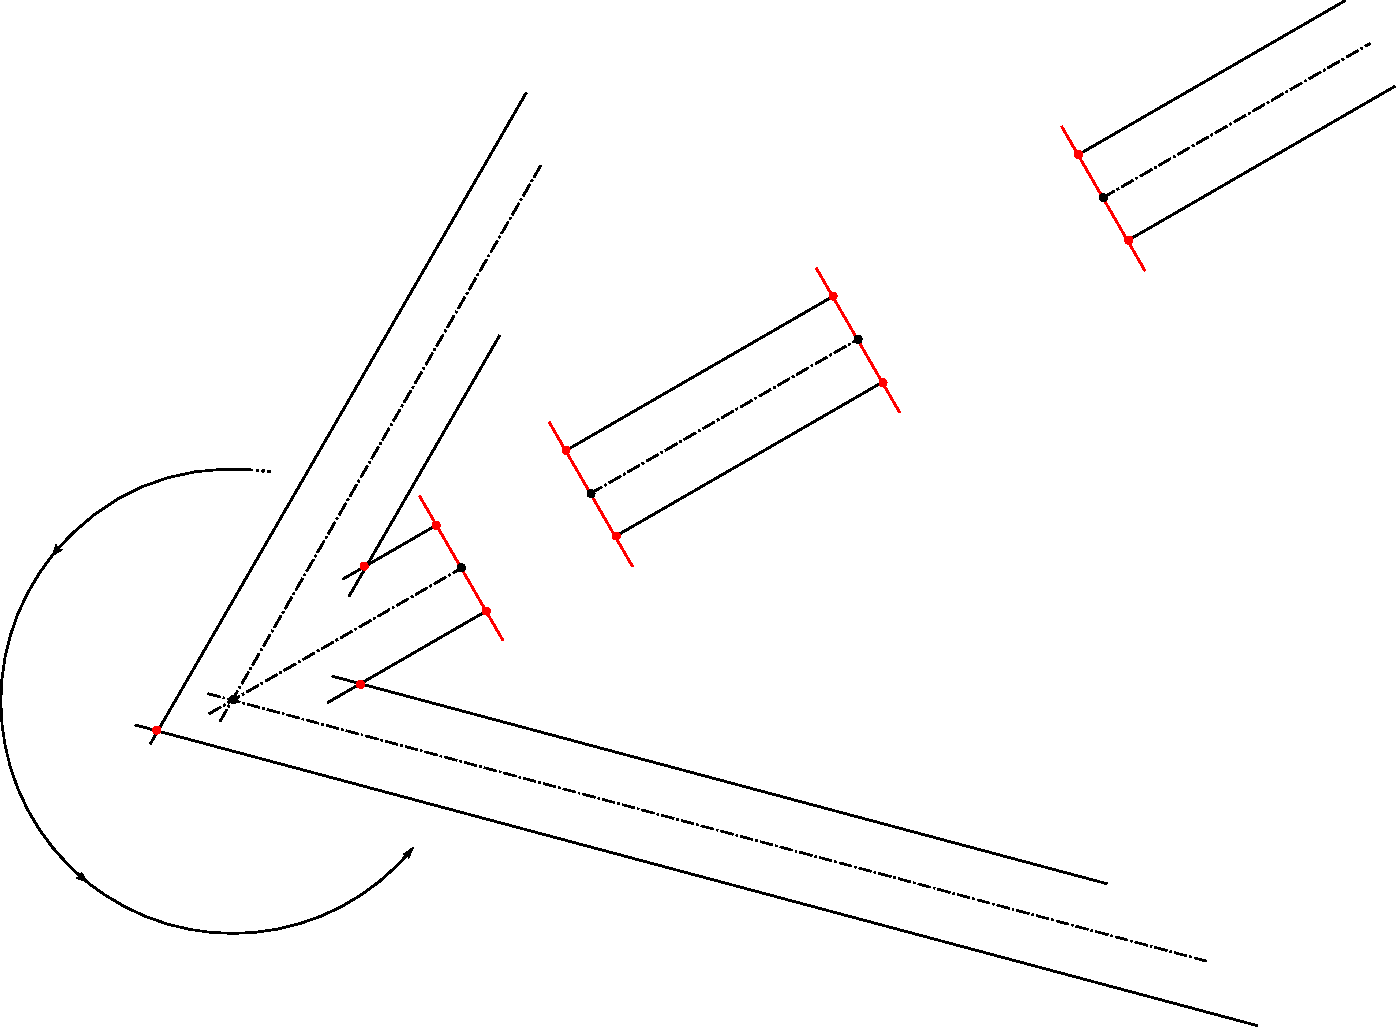
\includegraphics[width=0.9\textwidth]{figures/corners.pdf}
  \caption{Determinarea liniilor de contur pentru un Zid \label{figure:corner}}
\end{center}
\end{figure}

Destul de interesantă este metoda de desenare a zidurilor care, atît pentru 
desenarea reală cît şi pentru cea destinată editorului, aplică un algoritm de 
unire cu ceilalţi pereţi ce împart acelaşi colţ. Algoritmul calculează, 
printr-o parcurgere în sens trigonometric a tuturor zidurilor conectate la un 
colţ, interesecţia dintre muchiile interioare şi exterioare cu pereţii 
alăturaţi, aşa cum se poate vedea în Figura \ref{figure:corner}. Apoi se 
trasează liniile exterioare şi interioare pînă în punctele respective. Există, 
desigur, cazuri limită în care liniile trebuie eliminate datorită faptului că 
intersecţia depăşeşete dimensiunea reală a zidului şi atunci linia ar fi 
desenată de fapt în afara conturului zidului respectiv.

Zidurile sunt responsabile şi de desenarea tuturor Caracteristicilor aflate pe 
zid. Pentru aceasta, conturul exterior al zidurilor trebuie întrerupt în locul
în care caracteristica urmează să fie desenată. Această decupare este îmbinată
cu algorimtul de detectare a intersecţiilor cu celelalte ziduri din colţ. pentru
fie care dintre laturile zidurilor, se calculează punctele de intersecţie dintre
punctele ce delimitează fiecare caracteristică şi muchiile zidurilor, cum am
arătat în Figura \ref{figure:corner}.

Apoi, în spaţiul vid creat de delimitările tuturor caracteristicilor, printr-o
transformare afină, se mută sistemul de coordonate rotit şi poziţionat în
punctul de start al fiecărei caracterstici. În final se apelează rutina de
desenare a caractersticii, fie cea reală sau cea pentru editare, după caz.

\subsection{WallFeature}

Feature este clasa care marchează toate caracteristicile ce pot apărea pe un
Zid. Nu vom repeta enumerarea lor de la Secţiunea \ref{section:features}, ci vom
încerca să prezentăm modalitatea în care am implementat funcţionalitatea
acestora.

Practic, pentru fiecare caracteristică, cum am arătat la secţiunea precedentă,
zidul este prevăzut cu o cavitate în care desenarea este lăsată pe baza
caracteristicii. Dacă caracteristica nu ocupă întregul volum al zidului în zona
respectivă, este responabilitatea ei să ``cîrpească'' înapoi zidul, cum este
cazul ferestrelor, care lasă intact peretele în partea inferioară şi superioară
ferestrei în sine, sau la fel pentru uşi care au un spaţiu pînă la tavan.

Fiecare caracteristică trebuie să ofere propria reprezentare grafică, însă ele
sunt scutite de nevoile calculaţiilor poziţionale\footnote{Precum nu sunt
scutite zidurile, al căror algoritm de determinare a muchiilor implică calcule
complexe}, datorită faptului că zidurile aplică o transformare afină înainte de
iniţierea procedurii de desenare a caracteristicii, mutînd spaţiul de coordonate
în punctul de start al caractersticii şi cu rotaţia corespunzătoare.

\subsection{Decoration}

Decoraţiunile sunt componente independente de celelalte elemente de model, ce
sunt desenate poziţional direct de către model (precum zidurile). Simplitatea
lor implică puţine dificultăţi tehnice. Fiecare dintre ele a trebuit însă
proiectată cu grijă pentru a reda modelul reprezentat cît mai aproape posibil de
imaginea reală.

Cum este valabil şi pentru ziduri, nu se face detectare a suprapunerilor peste
alte obiecte, fiind astfel posibil ca diverse decoraţiuni să se suprapună peste
altele sau peste ziduri. O implementare rudimentară ar putea evita cele mai
multe din situaţiile de suprapunere, folosind funcţiile de suprapunere
implementate de fiecare obiect în parte.

\section{Editorul OpenGL}
\label{section:impl-editor}

\subsection{Integrarea cu Eclipse}
Editorul OpenGL este un editor pentru Eclipse RCP, şi respectă standardele
pentru un editor de acest fel. De aceea, el poate fi folosit ca orice alt editor
(i.e. Un editor de text pentru surse Java) în cadrul unei aplicaţii Eclipse. El
este integrat cu Eclipse şi se marchează ca editor standard pentru fişiere de
tip .ocm\footnote{Extensia standard a fişierelor acestui proiect: OpenCad.org
Model}.

Desigur, diferenţa majoră faţă de alte editoare întîlnite în Eclipse este că
prezentarea sa nu se face prin intermediul unui control de editare de text, ci
printr-o suprafaţă de desenare OpenGL. Cea mai mare parte a pragurilor care au
trebuit trecute în implementarea acestei aplicaţii au derivat din această
caracteristică deosebită a editorului nostru.

Editorul are o sursă de selecţie şi paginator de conţinut, a căror descriere o
vom prezenta în \ref{section:impl-selecta}. Prin această componentă, spunem că
Editorul OpenGL este integrat perfect cu Eclipse RCP, beneficiind (poate
beneficia astfel) de toate facilităţile pe care le are de oferit această
platformă.

\subsection{Plugin-ul OpenGL pentru SWT}
Editorul OpenGL este primul loc al aplicaţiei unde avem de aface cu plugin-ul
pentru OpenGL şi SWT. Deşi a fost scris special pentru Eclipse, acest plugin a
necesitat o extensivă testare şi configurare pentru funcţionarea corectă alături
de platforma Eclipse.

Plugin-ul de OpenGL funcţionează pe baza unei suprafeţe de desenare\footnote{O 
clasă numită GLCanvas}. În cadrul unei aplicaţii pot exista mai multe astfel de 
suprafeţe, \footnote{În cazul nostru era strict necesar existenţa a mai mult de 
o astfel de suprafaţă, datorită posibilităţii de a avea mai multe editoare, şi 
posibilitatea de a avea simultan Vizualizarea 3D} dar în orice moment o 
instrucţiune OpenGL nu poate desena decît într-o singură anume astfel de 
suprafaţă, desemnată printr-o rutină de selectare. Prima implementare (cea 
directă) a avut ca rezultat ``scurgerea'' de diverse efecte şi secţiuni din 
desen dintr-o suprafaţă în alta, datorită problemelor de sincronizare datorate 
de faptul că Eclipse RCP execută diverse operaţiuni în fire de execuţie 
diferite, care executau simultan instrucţiuni OpenGL fără o determinare precisă 
a suprafeţei în care ele desenau. Soluţia a fost sincronizarea diverselor 
metode din Editor şi Vizualizarea faţă de un punct fix, şi în cadrul zonei 
sincronizate să se selecteze (şi astfel să fie totdeauna determinată) suprafaţa 
de desenare.

\subsection{Maşina de stări}
Pentru implementarea maşinii de stări am folosit o stivă în vîrful căreia stătea
totdeauna starea activă\footnote{Am explicat funcţionarea Maşinii de stări în
Secţiunea \ref{section:machine}}.

Întreg comportamentul editorului este modelat prin intermediul acestor stări.
Pentru preluarea şi retragerea controlului anumitor stări asupra suprafeţei de
editare, se folosesc metode de aflare a unor obiecte de tratare a evenimentelor
pentru diverse evenimente ale editorului. Tipurile de obiecte de tratare sunt
prezentate în Tabela \ref{table:state-events}.

\begin{table}
\begin{tabular}{{|\col{0.28}|\col{0.68}|}}
\hline
\textbf{Clasă} & \textbf{Descriere Funcţionare}
\\ \hline
KeyListener & Poate interpreta orice apăsare de tastă (sau respectiv eliberare
de tastă, prin intermediul unui cod care indentifică unic orice tastă)

\\ \hline
MouseListener & Interceptează apăsările butoanelor mausului, fie cu click simplu
sau dublu, fiind capabil să reacţioneze la toate aceste evenimente, avînd
cunoştinţe asupra zonei în care mausul a fost apăsat.

\\ \hline
MouseMoveListener & Tratează orice mişcare a mausului în suprafaţa editorului şi
poate executa o rutină incrementală la fiecare deplasare a mausului.

\\ \hline
MouseTrackListener & Poate intercepta evenimentele de intrare a mausului, de
ieşire a acestuia şi starea de deplasare deasupra suprafeţei editorului.

\\ \hline
MouseWheelListener & Interceptează orice mişcare a rotiţei mausului pentru a
reacţiona în funcţie de viteza de rotaţie şi poziţia mausului în acel moment. De
notat că acest tip de eveniment nu are o clasă proprie ci se lucrează direct cu
interfaţa generică Listener.

\\ \hline
\end{tabular}
\caption{Tipurile de evenimente ce pot fi tratate de o stare a editorului
\label{table:state-events}}
\end{table}

\subsection{Interacţiunea cu utilizatorul. Prezentarea 2D}
Editorul OpenGL poate interacţiona prin intermediul mausului cu orice obiect din
model ce suportă acest comportament. Pentru aceasta, editorul trebuie să reţină
în orice moment caracteristicile zonei care este desenată pe ecran, adică
punctul de start, dimensiunile în coordonate model ale ferestrei de afişare. La
fiecare interacţiune cu mausul, coordonatele ecran sunt transformate în
coordonate model cu ajutorul acestor informaţii.

Editorul are, de asemenea, capacitatea de a modifica valorile de vizualizare
într-un mod intuitiv, care-i permite să vizualizeze diverse detalii ale
modelului la diverse scări de mărire. Utilizatorul poate controla aceste
caracteristici cu ajutorul stării de navigare, în care tragerea suprafeţei de
editare mută punctul de start iar scroll-ul cu rotiţa modifică scara desenului.

De asemenea, redimensionarea ferestrei va mări suprafaţa de desenare după un
algoritm special. Pe scurt, acest algoritm încearcă să păstreze aceeaşi mărire
relativă a modelului\footnote{Se păstrează aceeaşi cantitate de detalii în
desen}, la acelaşi aspect al ferestrei de vizualizare. La modificare aspectului,
cantitatea de detalii va ramîne constantă în zona pătratică a desenului,
crescînd înspre zonele unde modificarea aspectului scoate la iveală noi zone din
model.

\section{Vizualizarea 3D}
\label{section:impl-view}

\subsection{Integrarea cu Eclipse}
Vizualizarea 3D este o Vizualizare Eclipse standard. Ca şi în cazul editorului,
particularitatea componentei create de noi este că foloseşte pentru
reprezentarea conţinutului o suprafaţă de desenare OpenGL. Diferenţa
fundamentală faţă de Editor este căm în cazul vizualizării, utilizatorul nu
poate modifica modelul de lucru prin interacţiunea cu controlul respectiv.
Astfel, se reduce mult din nevoile şi calculaţiile necesare (nu avem nevoie nici
de mecanismul de stări prezent la editor). Vizualizarea este doar o modalitate
foarte bună de vizualizarea tridimensională a modelului final.

\subsection{Prezentarea 3D}
Deşi toate rutinele de desenare sunt prezente în fiecare componentă a modelului
în parte, vizualizarea are însă totuşi responsabilitatea de a face unele
operaţii pentru suprafaţa de desenare.

În principal, are aceleaşi responsabilităţi de sincronizare de threaduri pe care
le are şi Editorul. Deşi nu poate exista decît o singură vizualizare, motorul de
desenare OpenGL interacţionează în acelaşi fel cu toate componentele care doresc
să deseneze pe o suprafaţă OpenGL.

De asemenea, vizualizarea are răspunderea de a seta datele proiecţiei, în
funcţie de unghiul de privire şi punctul de centru pe care utilizatorul le poate
modifica cu ajutorul mausului. Pentru controlul acestor coordonate, vizualizarea
captează evenimentele mausului întocmai ca o stare a editorului şi tratează
diverse mişcări ale mausului în sensul modificării parametrilor de vizualizare.

\section{Sursa de selecţie}
\label{section:impl-selecta}
Sursa de selecţie, reprezentată de clasa GLEditorOutlinePage serveşte în 
principal vizualizării de structură, prezentată la \ref{section:impl-outline}. 
Însă în acelaşi timp, serveşte unui scop similar sincronizării cu Vizualirea 
3D. Principala ei funcţie este să anunţe tuturor celor înscrişi schimbarea 
selecţiei în editor. Schimbarea selecţiei poate avea mai multe 
surse\footnote{i.e. Vizualizarea structurii poate schimba selecţia}, şi deci şi 
editorul în sine ascultă acest serviciu. Pentru aceasta, el trebuie să se
protejeze la a reacţiona în lanţ la acţiunea de schimbare a
selecţiei\footnote{El cînd schimbă selecţia anunţă serviciul, care apoi îl
anunţă pe el, el schimbă selecţia şi anunţă din nou, etc.}.

În acelaşi timp clasa menţionată serveşte ca sursă de conţinut pentru
Vizualizarea de structură. Arborii în SWT sunt structuri abstracte, care separă
conţinutul de prezentare, şi partea lor de sursă de date este tocmai această
clasă.

\section{Vizualizarea structurii}
\label{section:impl-outline}

Vizualizarea de structură se bazează în principal pe Sursa de selecţie, descrisă
la \ref{section:impl-selecta}. În general, toate editoarele din Eclipse
beneficiază de această componentă, şi utilizatorul se aşteaptă ca în cadrul ei
să vizualizeze toate componentele logice într-o structura naturală.

În cazul de faţă, se prezintă toate primitivilele şi conexiunile dintre ele,
într-o structură arborescentă. Deşi legăturile dintre primitive sunt mai
complexe, se reprezintă într-o versiune simplificată şi uşor de înţeles pentru
utilizator.

Conţinutul efectiv al vizualizării este dat de sursa de selecţie, prezentată la
\ref{section:impl-selecta}. Vizualizarea de structură este doar o componentă
standard a Eclipse RCP, particularizată prin conectarea cu sursa de selecţie.

\section{Particularizările interfeţei Eclipse}
